\documentclass{article}

% Call the style package
\usepackage[english]{babel}

\usepackage{graphicx} 
\usepackage{amsmath}
\usepackage{amssymb}
\usepackage{amsfonts}
\usepackage{amstext}
\usepackage{amsthm}
\usepackage[
sorting=none
]{biblatex}
\usepackage{csquotes}
\addbibresource{biblio.bib}
    
\title{VR-Diskotek}
\author{Joan S. Gerard S., ULB}
\date{January 13th, 2019}
\usepackage{subcaption}

\begin{document}

\maketitle

\section{Project Description}

% Brief description of the problem
The goal of this project is to apply what we have learned during classes on a project using OpenGL together with C++. VR-Diskotek is a project in which a set of lights is used to recreate a dance club environment in a closed room that contains some models. Notice that this project was made following three main websites for learning OpenGL: LearnOpenGL\cite{web:learnopengl},  OpenGLTutorial\cite{web:opengl-tuto}, and ThinMatrix Youtube Channel\cite{web:thinMatrix}.

\begin{figure}[htp]
    \centering
    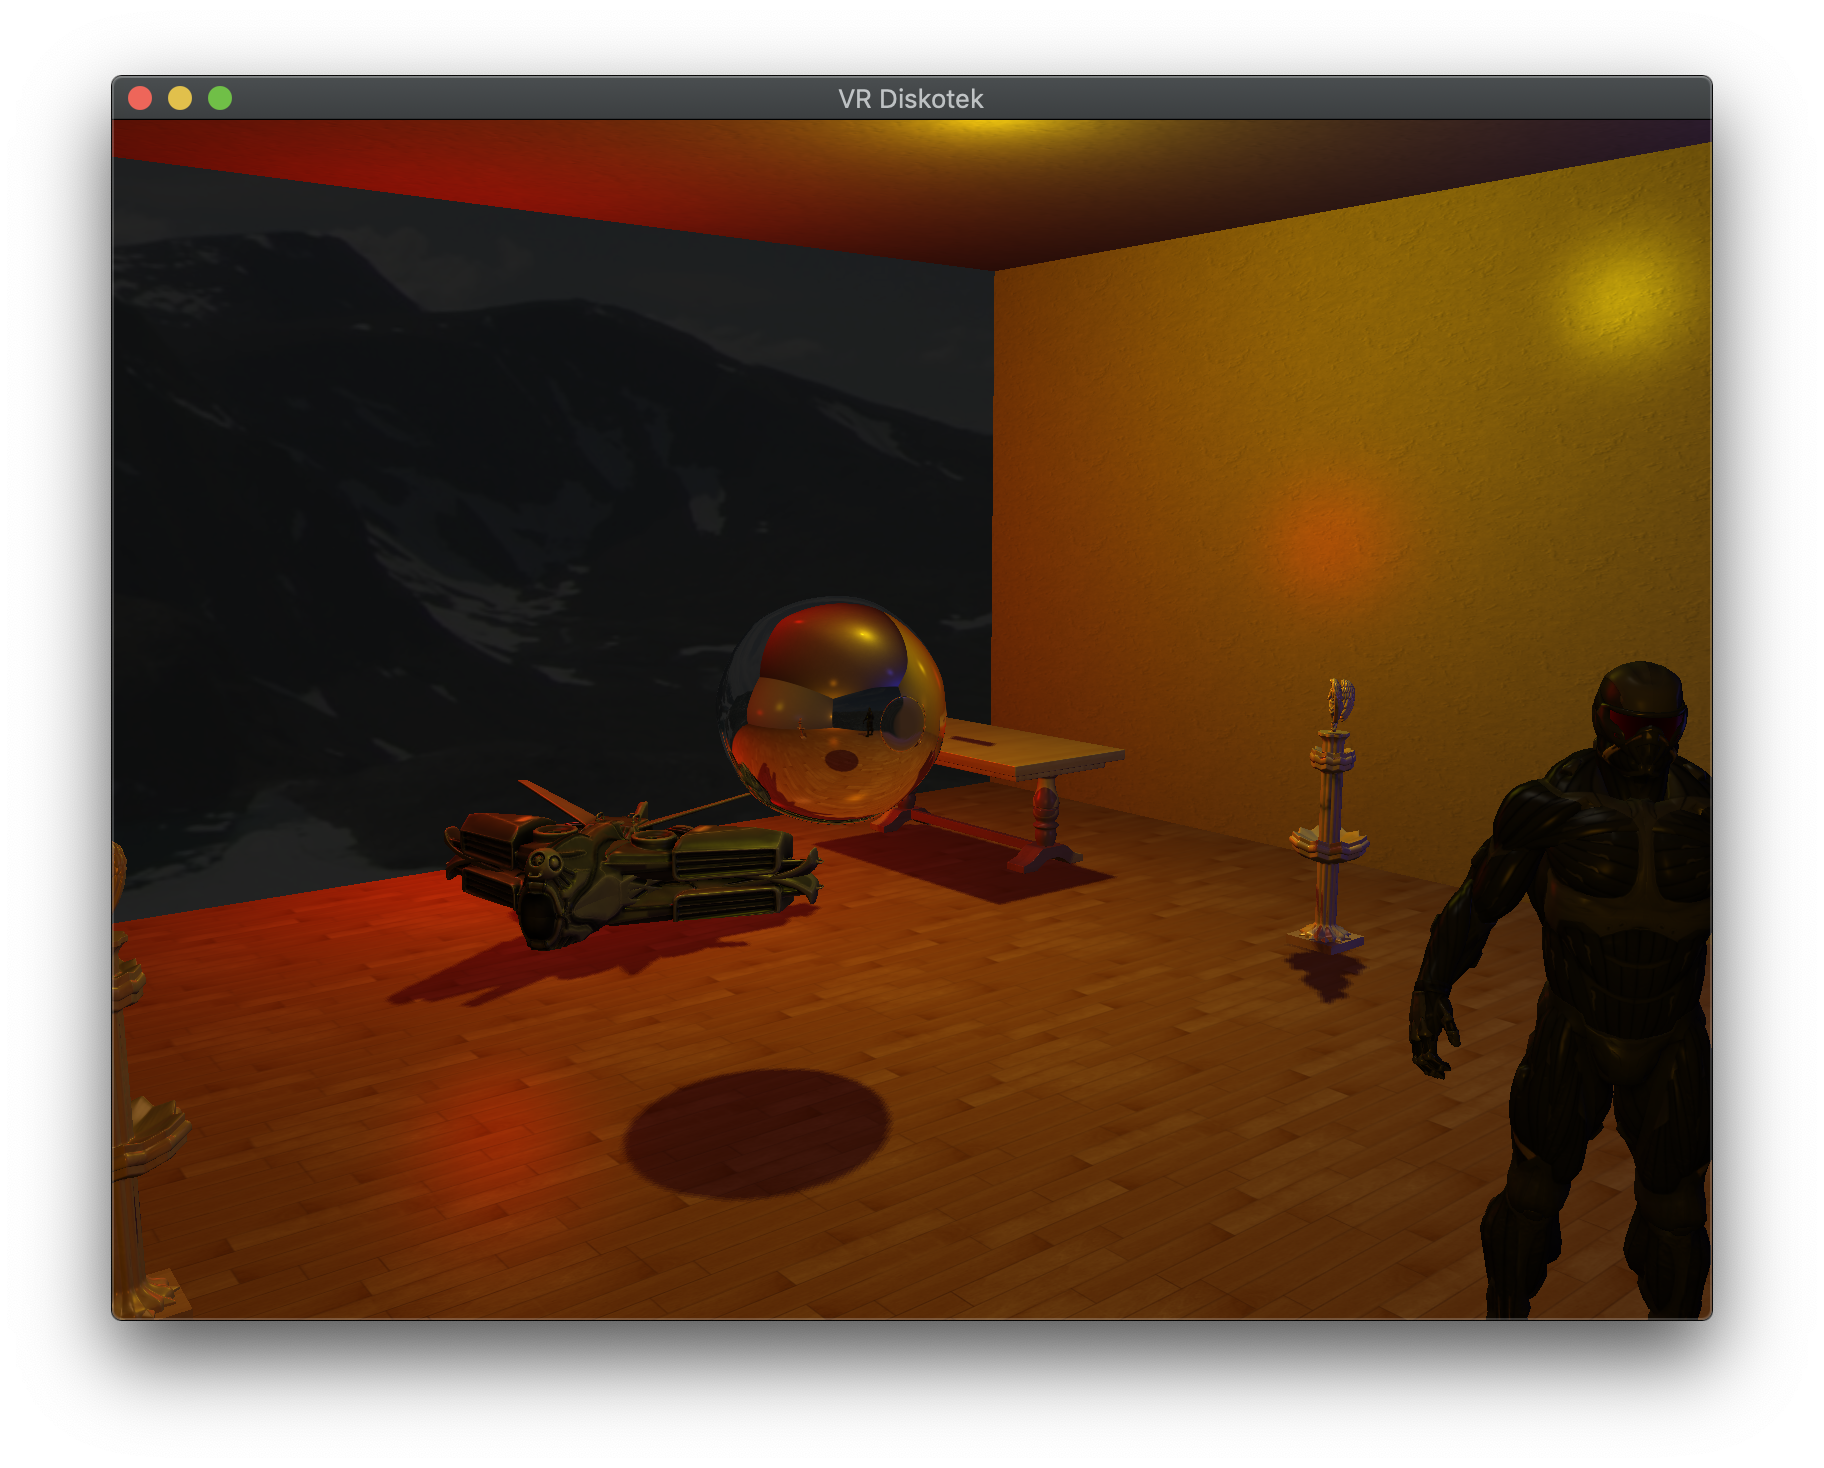
\includegraphics[width=10cm]{ex.png}
    \caption{VR-Diskotek: Dance Club Mode}
    \label{fig:galaxy}
\end{figure}

\section {Components}
In this section all the components used in this project will be mentioned but not detailed.
\begin{itemize}
  \item A set of four lights: three static on the walls and one dynamic near the roof. Press H key to change the light configuration. There are three configurations: dance club mode, rock concert mode and techno club mode (see video for more details).
  \item Two types of light: Directional and Point light each one configured with Ambient, Difusse and Specular shading. Point lights have an attenuation factor of
  $\frac{1.0}{K_c + K_l*d + K_q*d^2}$ where $K_c$ is a constant term, $K_l$ a linear term, $K_q$ the quadratic term and $d$ the distance from the fragment to the light source. Thus further the light source is from the model, less the impact of the light on it.
  \item A total of 6 models with textures are loaded: the nanosut, a fountain (x2), a table, a laptop, an intergalactic ship and a giant ball. The nanosut and the intergalactic ship turn around it's on position.
  \item The two fountains have a particle system that simulates water falling up/down.
  \begin{figure}[htp]
        \centering
        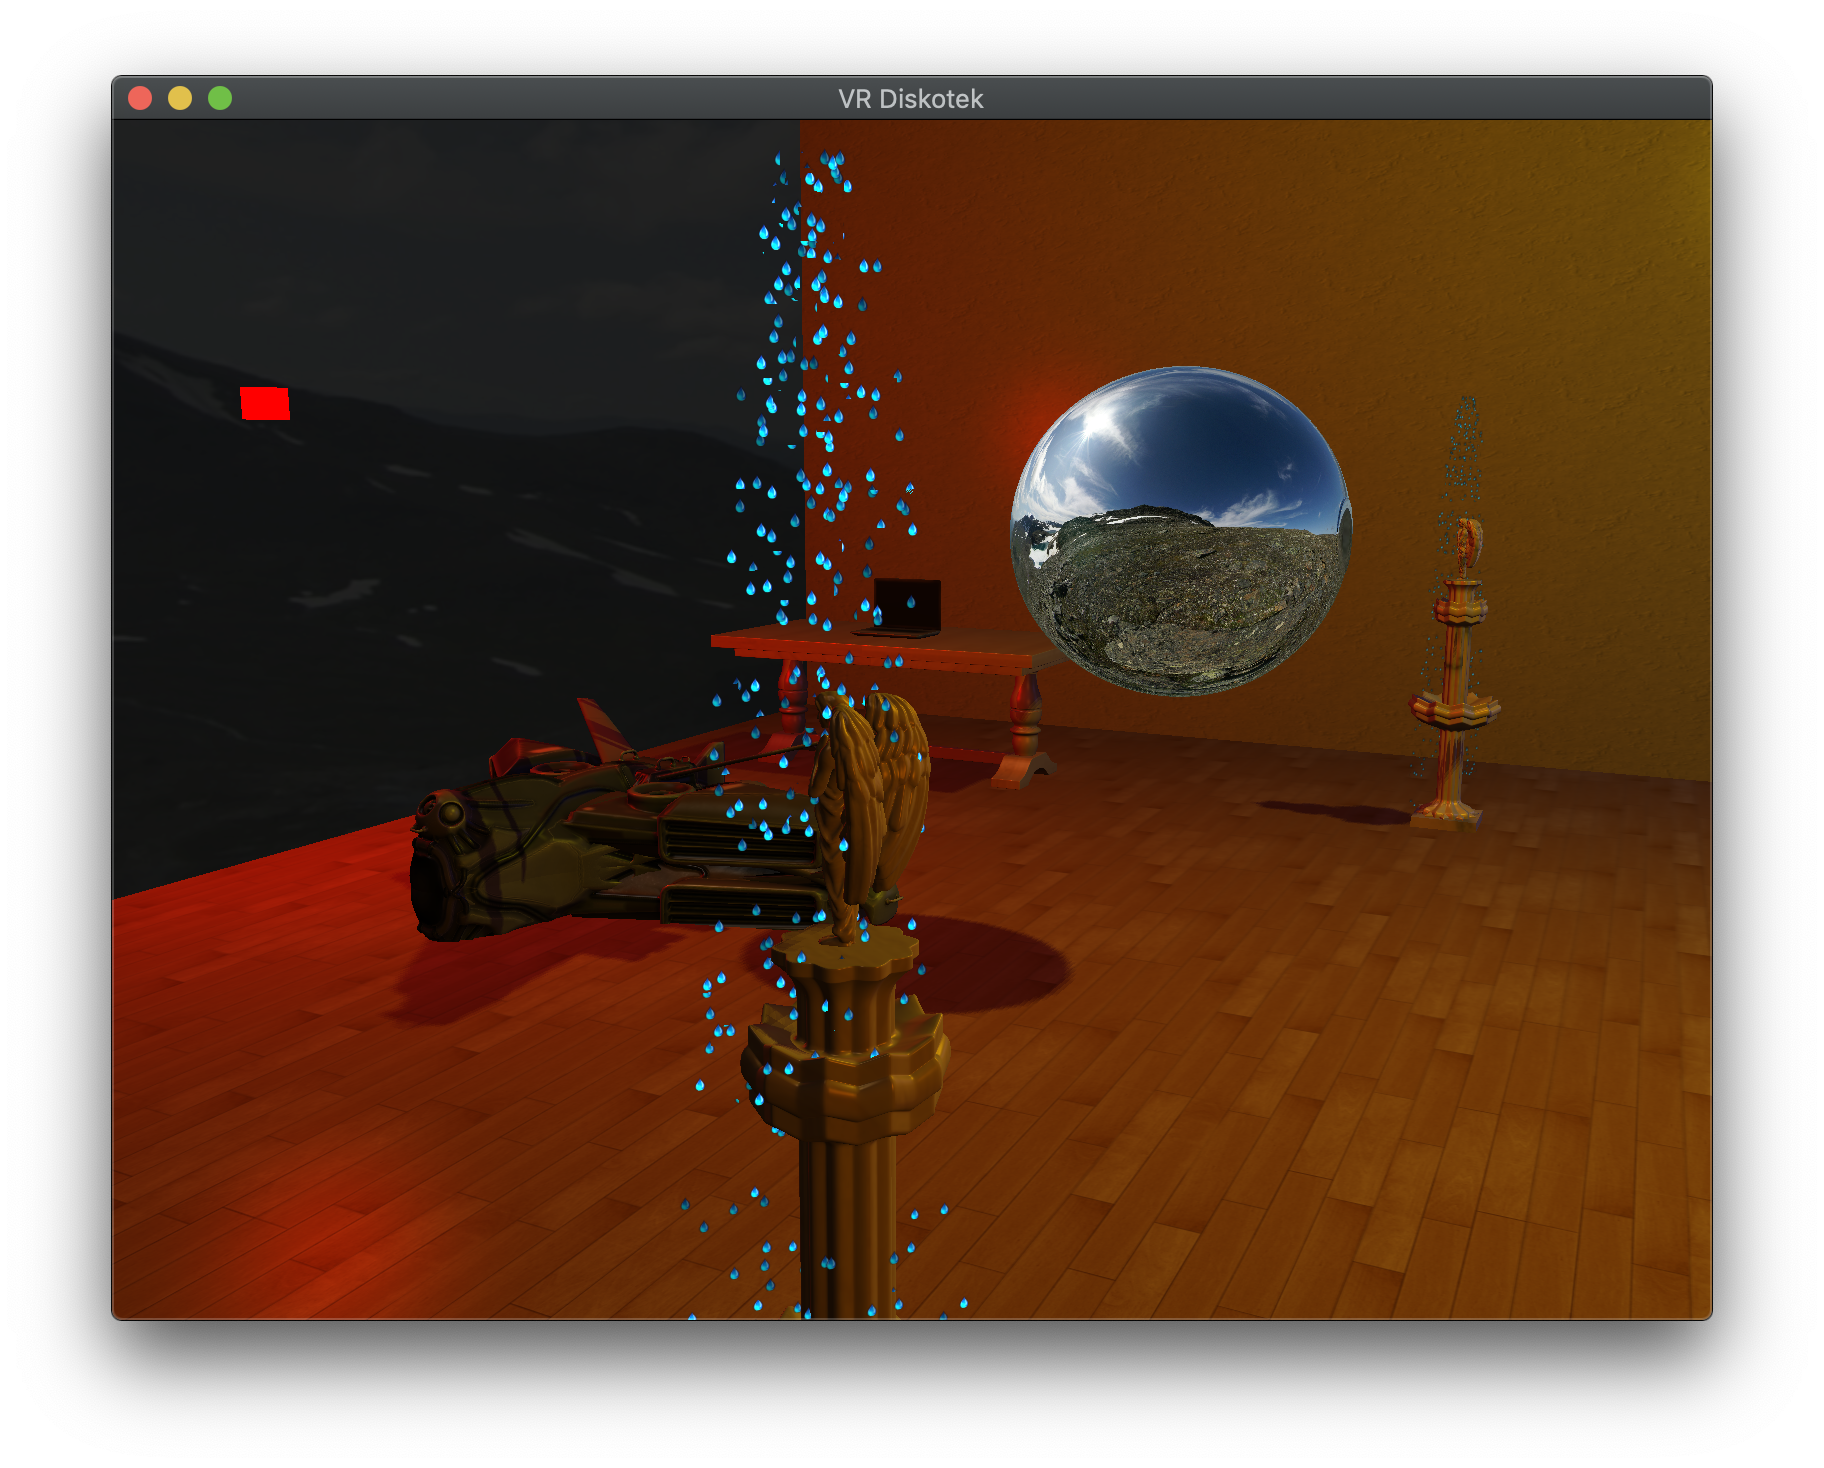
\includegraphics[width=10cm]{particles.png}
        \caption{Particle System}
        \label{fig:galaxy}
    \end{figure}
    
 \item The giant ball has a Dynamic Environment Map that reflects the entire scene on it. It can be disabled/enabled pressing the J key. 
 \begin{figure}[htp]
        \centering
        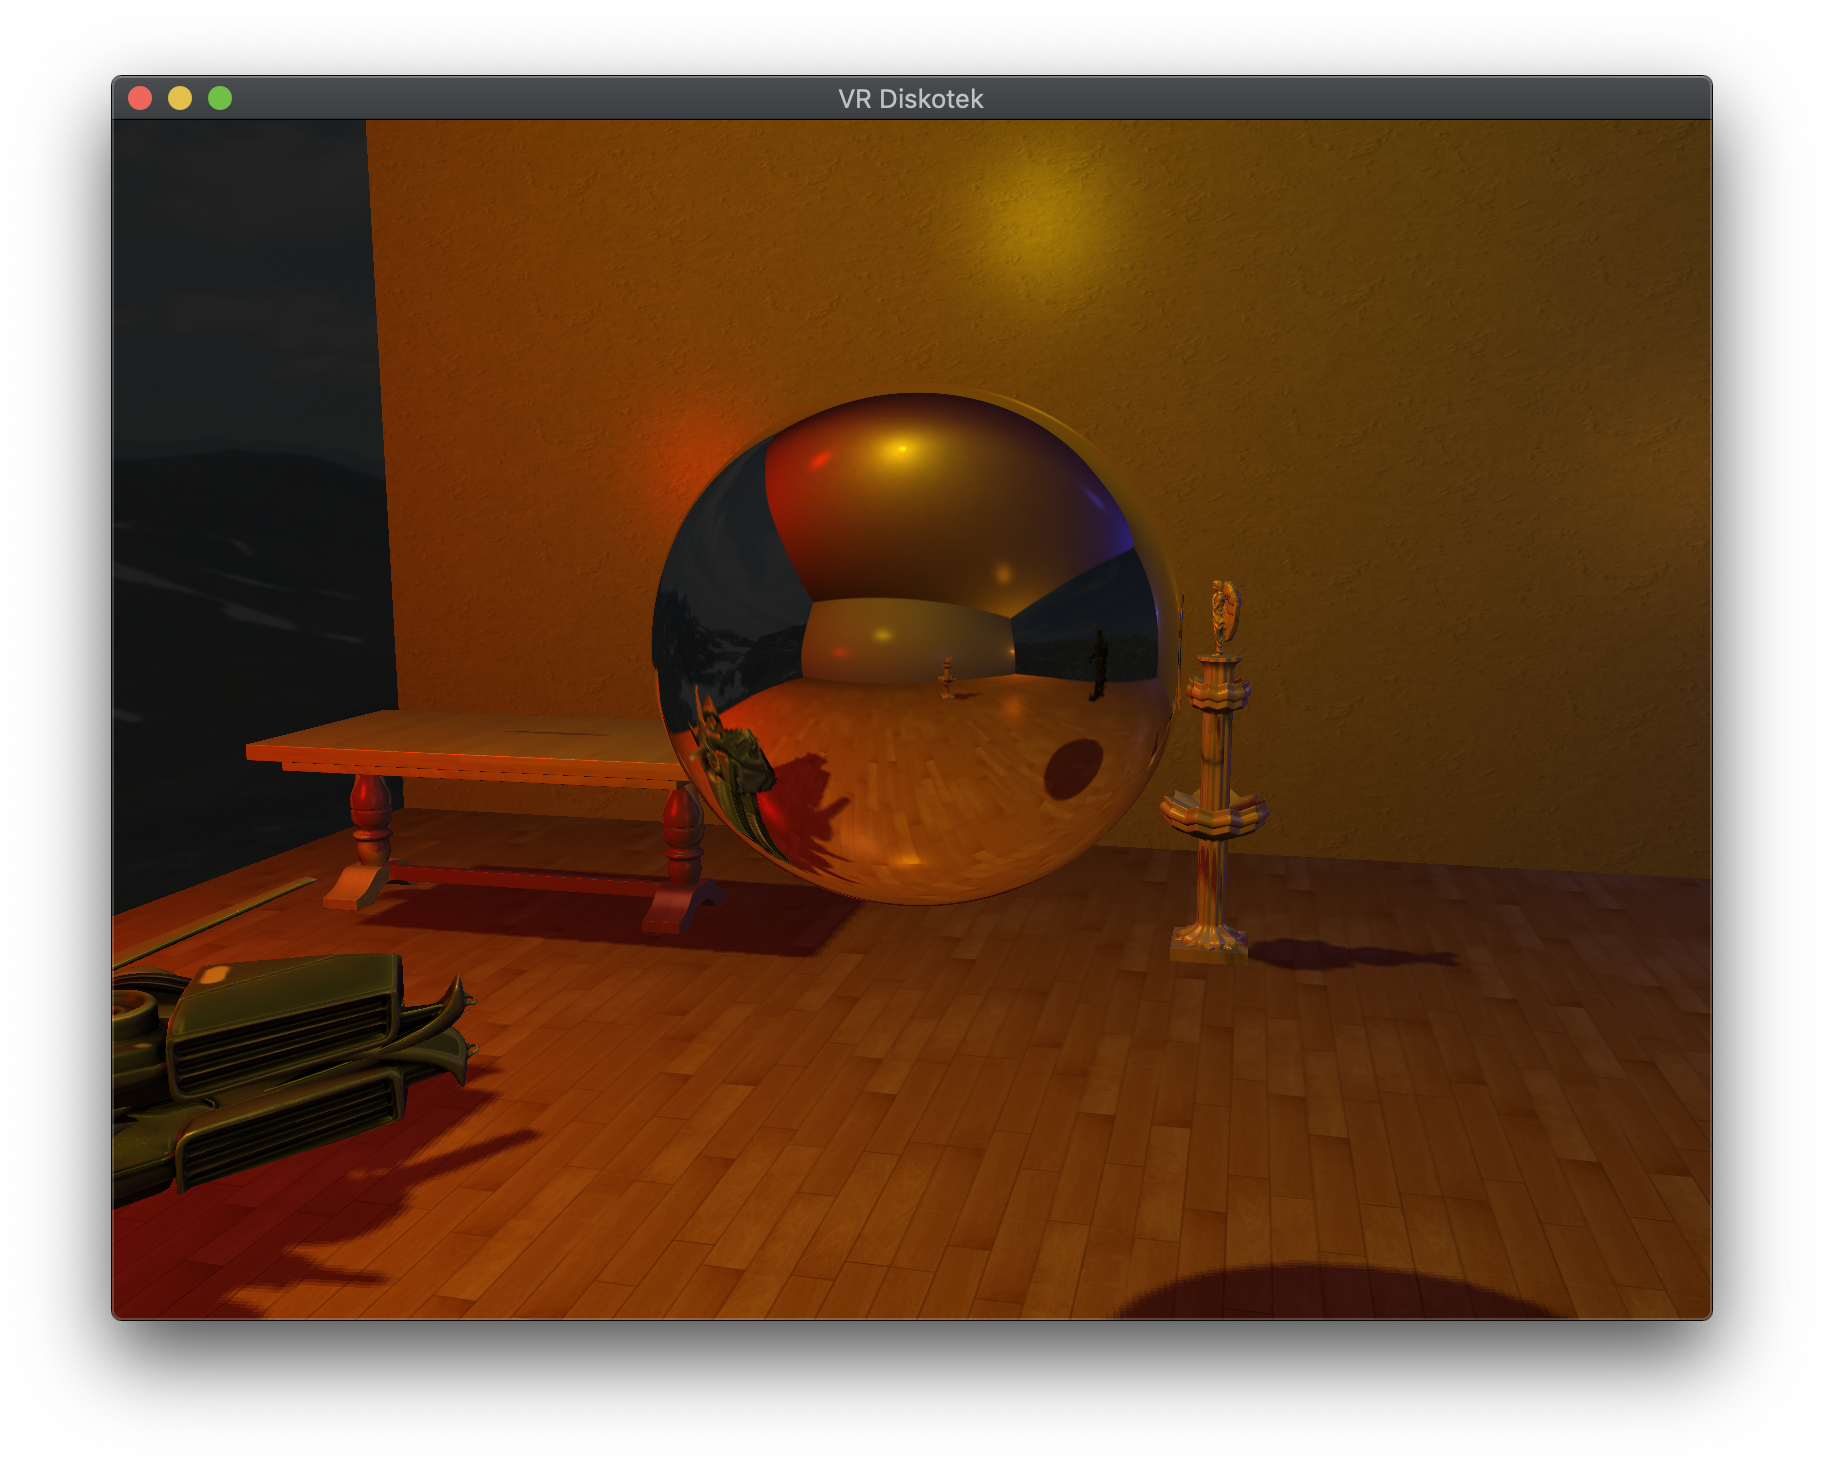
\includegraphics[width=10cm]{mirrow.png}
        \caption{Mirror Effect}
        \label{fig:galaxy}
    \end{figure}
    \item There is a cubemap loaded on the scene that can be seen through the 
    black windows.
    \item The objects have shadows projected according to the light source moving on top of the scene.
\end{itemize}

\section{Mirror Effect}
In order to obtain the mirror effect the scene needs to be drawn from the point of view of the giant ball looking to 6 directions: left, right, up, down, front and back. This technique draws the scene into the frame buffer and then it constructs a cubemap which is used as a texture for the giant ball. Before drawing the scene into the frame buffer, the viewport needs to be set to (in this case) 128 to obtain
a low resolution image of the environment. The field of view needs to be set to 90 degrees and the aspect ratio to one. This is for having the entire scene rendered. The performance of this technique may be improved using face culling.

\section{Particles System}
A particles system is used to simulate the water fountain. A total of 5000 particles is used. Each particle has a color, a speed, a position and a life limit.
At each step of the rendering loop a new set of particles is created replacing the ones that are already dead (whose $life < 0$) to avoid using more memory than needed.
The particles start with the speed vector pointing up added to some random vector to avoid taking the same direction. Then their speed is updated adding the gravity vector to let the particle going up and then down. The particle's life is set to 4 seconds only. Then each alive particle is rendered individually. The performance of this method could be improved using $glDrawArraysInstanced$ instead of $glDrawArrays$ which calls the last one $n$ times but it is supposed to be faster.

\section{Shadow Map}
For creating the shadows it is needed to render the scene into the depth buffer from the light's perspective and thus generating a depth map that will be used to calculate whether a fragment should be in a shadow or not. Some problems are solved while calculating shadowing like Shadow Acne, Peter panning, jagged blocky edges using common techniques like PCF for the later.
\printbibliography

\end{document}
